%!TEX root = ../msc_thesis.tex

\chapter{Active Learning}
\label{ch:active_learning}

%%%%%%%%%%%%%%%%%%%%%%%%%%%%%%%%%%%%%%%%%%%%%%%%%%%%%%%%%%%%%%%%%%%%%%%%%%%%%%%%%%%%%%%%%%
%%%%%%%%%%%%%%%%%%%%%%%%%%%%%%%%%%%%%%%%%%%%%%%%%%%%%%%%%%%%%%%%%%%%%%%%%%%%%%%%%%%%%%%%%%
%%% AL
%%%%%%%%%%%%%%%%%%%%%%%%%%%%%%%%%%%%%%%%%%%%%%%%%%%%%%%%%%%%%%%%%%%%%%%%%%%%%%%%%%%%%%%%%%
%%%%%%%%%%%%%%%%%%%%%%%%%%%%%%%%%%%%%%%%%%%%%%%%%%%%%%%%%%%%%%%%%%%%%%%%%%%%%%%%%%%%%%%%%%

% \section{Active Learning}

An active learning problem is one in which the learner is able to select its own training data so that the performance will be better with less training data. This is attractive because many times, labeled data is expensive or hard to acquire, hence the desire to use the labeled data as efficiently as possible.

For example, in supervised learning, a modeler may have access to a lot of unlabeled data and few labeled data which are expensive to label my human annotators. An active learning task would be to train a model $\hat{f}$ with an initial set of labeled data $\mathcal{L}$. Afterwards, the learner can choose new data points $\boldsymbol{x}^*$ from an unlabeled pool of data $\mathcal{U}$, ask to an \textit{oracle} (e.g., a human annotator) what the corresponding output $y^*$ is, and then add the pair $(\boldsymbol{x}^*, {y}^*)$ to the training data, and this process may be repeated until a certain criteria are met, with the training set increasing in size in every iteration. Figure \ref{fig:Active_Learning_Cycle} shows this cycle in a diagram. The main goal of active learning is to select which $\boldsymbol{x}^*$ to incorporate to the training data \cite{cohn1996active}. In the end, it is expected that this procedure leads to a better predictive performance than randomly selecting new observations to add to the training data.

\begin{figure}[H]
    \centering
    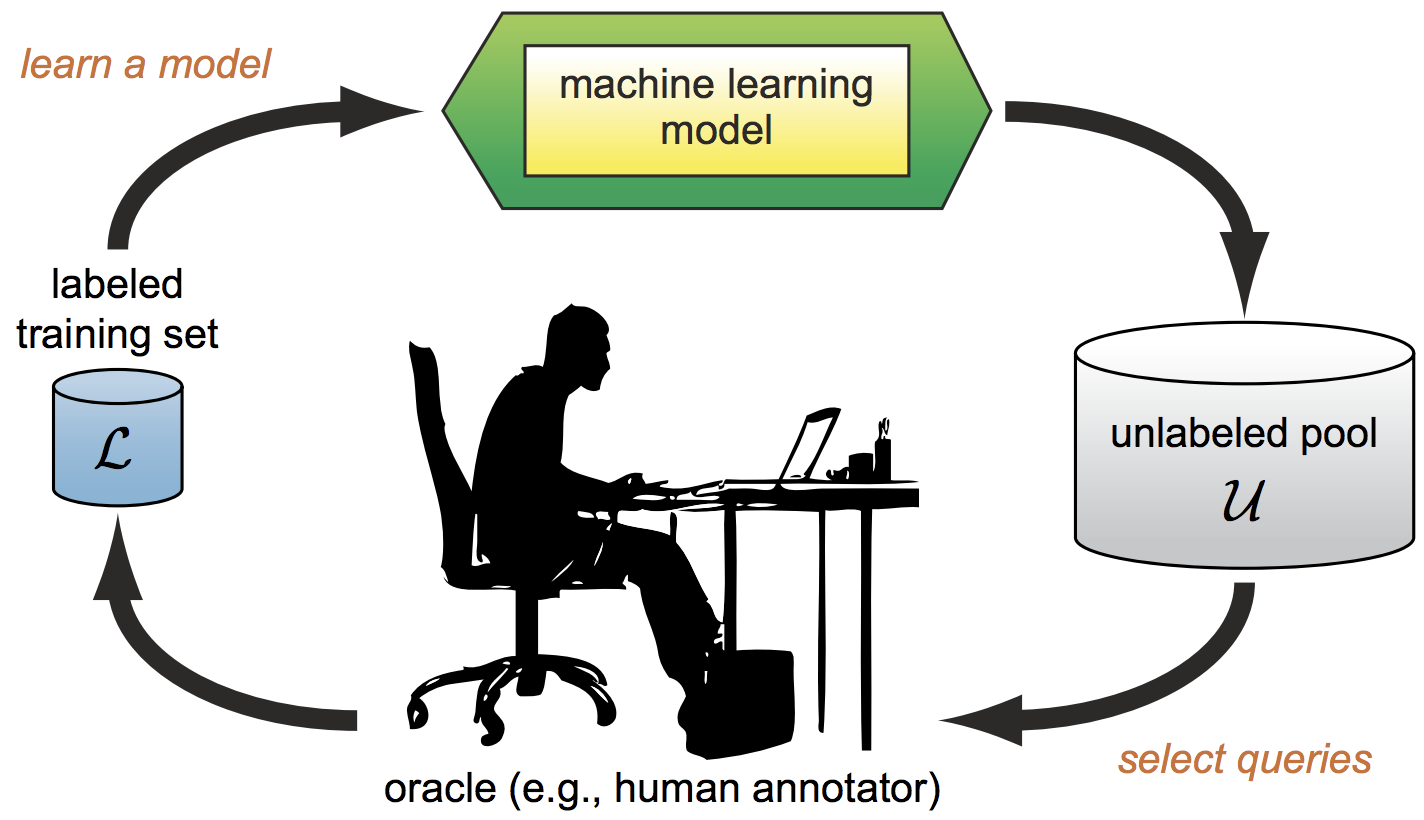
\includegraphics[width=0.8\textwidth]{Active_Learning_Cycle}
    \caption{Active Learning cycle. A model is trained from the labeled data $\mathcal{L}$, data points are taken from the unlabeled pool of data $\mathcal{U}$, labeled by an oracle and then added to the training set of labeled data $\mathcal{L}$ in order to retrain the model and continue the cycle. Image taken from \cite{settles.tr09}.}
    \label{fig:Active_Learning_Cycle}
\end{figure}

% For example, in a supervised learning problem where there is a data set with features $\boldsymbol{X}$ and response variable $\boldsymbol{y}$. First we train a model $\hat{f}$ with the data that we have, afterwards the learner can choose new data $\boldsymbol{x}^*$ from an unlabeled pool of data, ask to an \textit{oracle} what the corresponding output $y^*$ is, and then add the pair $(\boldsymbol{x}^*, {y}^*)$ to the training data. The main goal of active learning is to select which $\boldsymbol{x}^*$ to incorporate to the training data \cite{cohn1996active}.

The type of active learning described before, in which there is a large collection of unlabeled data $\mathcal{U}$ and a small set of labeled data $\mathcal{L}$, is usually called \textit{pool-based sampling} \cite{settles.tr09}, and will be the main focus of this work. There are other types of Active Learning but, since they are not of interest to this work, they will not be discussed.

As mentioned before, in pool-based sampling, a model is trained with labeled training data from $\mathcal{L}$, and then, new data points are chosen to be labeled from the unlabeled data pool $\mathcal{U}$. The new data points are chosen using an \textbf{acquisition function} $a(x, \hat{f})$ that is usually based on the model's uncertainty about the prediction. The new observation $\boldsymbol{x}^*$ is chosen so that it maximizes the acquisition function of all the observations in the pool set. The role of the acquisition function is to evaluate the informativeness of each unlabeled data point.

The acquisition functions that will be used and compared in this work are four, and three of them use the posterior predictive distribution, particularly, the posterior predictive probability of an observation $\boldsymbol{x}^*$ having a label $y^*$ belonging to a class $c$, denoted as $p(y^* = c | \boldsymbol{X}, \boldsymbol{y}, \boldsymbol{x}^*)$. Naturally, because of the definition of these acquisition functions, they only work in classification problems.

\begin{enumerate}
  \item Predictive entropy:

  $\mathbb{H} \left[ y^* | \boldsymbol{X}, \boldsymbol{y}, \boldsymbol{x}^* \right] = - \sum_c p(y^* = c | \boldsymbol{X}, \boldsymbol{y}, \boldsymbol{x}^*) \log p(y^* = c | \boldsymbol{X}, \boldsymbol{y}, \boldsymbol{x}^*)$.

  \item Variation ratios: $1 - \max_y p(y^* | \boldsymbol{X}, \boldsymbol{y}, \boldsymbol{x}^*)$.

  \item Bayesian Active Learning by Disagreement (BALD):

  $\mathbb{H} \left[ y^* | \boldsymbol{X}, \boldsymbol{y}, \boldsymbol{x}^* \right] - \mathbb{E}_{p(\boldsymbol{\theta} | \boldsymbol{X}, \boldsymbol{y})} \left[ \mathbb{H} \left[ y^* | \boldsymbol{x}^*, \boldsymbol{\theta} \right] \right]$.

  \item Random: Choosing an observation uniformly random from the pool of unlabeled data $\mathcal{U}$.

\end{enumerate}

Note that predictive entropy and variation ratios can be used with a frequentist classifier because instead of using the posterior predictive distribution, one can use the predicted probability of each class. The BALD acquisition function, however, can only be used with a Bayesian classifier because in the case of a frequentist classifier, the result of this function is always zero. This is easy to see given the definition of the acquisition function
\begin{equation}
	\label{eq:bald_acq_func_def}
	% \mathbb{I}[y^*, \mathcal{W} | x, \mathcal{D}] =
  \mathbb{H} \left[ y^* | \boldsymbol{X}, \boldsymbol{y}, \boldsymbol{x}^* \right] -
    \mathbb{E}_{p(\boldsymbol{\theta} | \boldsymbol{X}, \boldsymbol{y})} \left[ \mathbb{H} \left[ y^* | \boldsymbol{x}^*, \boldsymbol{\theta} \right] \right],
\end{equation}
where $\mathbb{H} \left[ y^* | \boldsymbol{X}, \boldsymbol{y}, \boldsymbol{x}^* \right]$ is the predictive entropy, previously defined as
\begin{equation}
	\label{eq:entropy_acq_func_def}
  \mathbb{H} \left[ y^* | \boldsymbol{X}, \boldsymbol{y}, \boldsymbol{x}^* \right] = - \sum_c p(y^* = c | \boldsymbol{X}, \boldsymbol{y}, \boldsymbol{x}^*) \log p(y^* = c | \boldsymbol{X}, \boldsymbol{y}, \boldsymbol{x}^*).
\end{equation}

In the Bayesian case, one has a positive number of samples from the posterior predictive distribution, so the second part of equation \eqref{eq:bald_acq_func_def}, i.e., the expected value
$\mathbb{E}_{p(\boldsymbol{\theta} | \boldsymbol{X}, \boldsymbol{y})} \left[ \mathbb{H} \left[ y^* | \boldsymbol{x}^*, \boldsymbol{\theta} \right] \right]$
is approximated by averaging the predictive entropy of each predictive sample; this way the BALD acquisition function is computed by taking the difference of this quantity and the first part of equation \eqref{eq:bald_acq_func_def}.
In the frequentist case, there is only one point estimate, so that difference is zero, hence the BALD acquisition function is always zero.

If the data points in the pool of unlabeled data points $\mathcal{U}$ are in random order, then using BALD as an acquisition function with a frequentist classifier is equivalent to a random acquisition function because all data points in $\mathcal{U}$ have the same acquisition function value.

An example of the active learning cycle can be seen in figure \ref{fig:log_reg_AL_accuracies_plot}. This figure summarizes the results of a two class classification problem using a logistic regression model. Similarly to what was done in chapter \ref{ch:machine_learning}, a data set was generated with a data matrix $\boldsymbol{X} \in \mathbb{R}^{n \times 10}$ with $n = 1000$ such that $\boldsymbol{x_i^{(k)}} \sim N(0, 1)$ for each $i \in \left\{1, ..., n \right\}$ and $k \in \left\{1, ..., 10 \right\}$.
Then an auxiliary vector was computed, $p_i = \frac{1}{1 + \exp \left( - \sum_{k = 1}^{10} \theta_k x_i^{(k)}  \right)}$, with each $\theta_k$ created at random from a continuous uniform distribution from -5 to 5. Finally, the response variable $\boldsymbol{y}$ was built simulating Bernoulli random variables, such that $y_i \sim \mathrm{Bern}(p_i)$.

For the example, an initial random training set of 20 observations $\mathcal{L}$ was created, with 10 examples of each class. Of the 980 points that were not used, 300 were used as a validation set, and the remaining 680 points were used as the unlabeled pool set $\mathcal{U}$.
Then, 180 acquisition iterations were made, in each iteration training a logistic regression model, making predictions on the pool set $\mathcal{U}$, and use these predictions to compute the frequentist variation ratios and choose the data point with the highest value so that it would be added to the training set set $\mathcal{L}$. In order to remove sampling noise, this process was repeated 50 times, each time choosing different initial random training, validation and pool sets. The same was done using a random acquisition function to compare with the Active Learning setting.

Figure \ref{fig:log_reg_AL_accuracies_plot} shows the mean accuracy on the validation set in each acquisition iteration, with the light colors showing the 25-th and 75-th percentiles of the accuracies in each iteration. It is clear that using Active Learning leads to a better performance of the model with less data compared to a random sample from $\mathcal{U}$.

\begin{figure}[H]
    \centering
    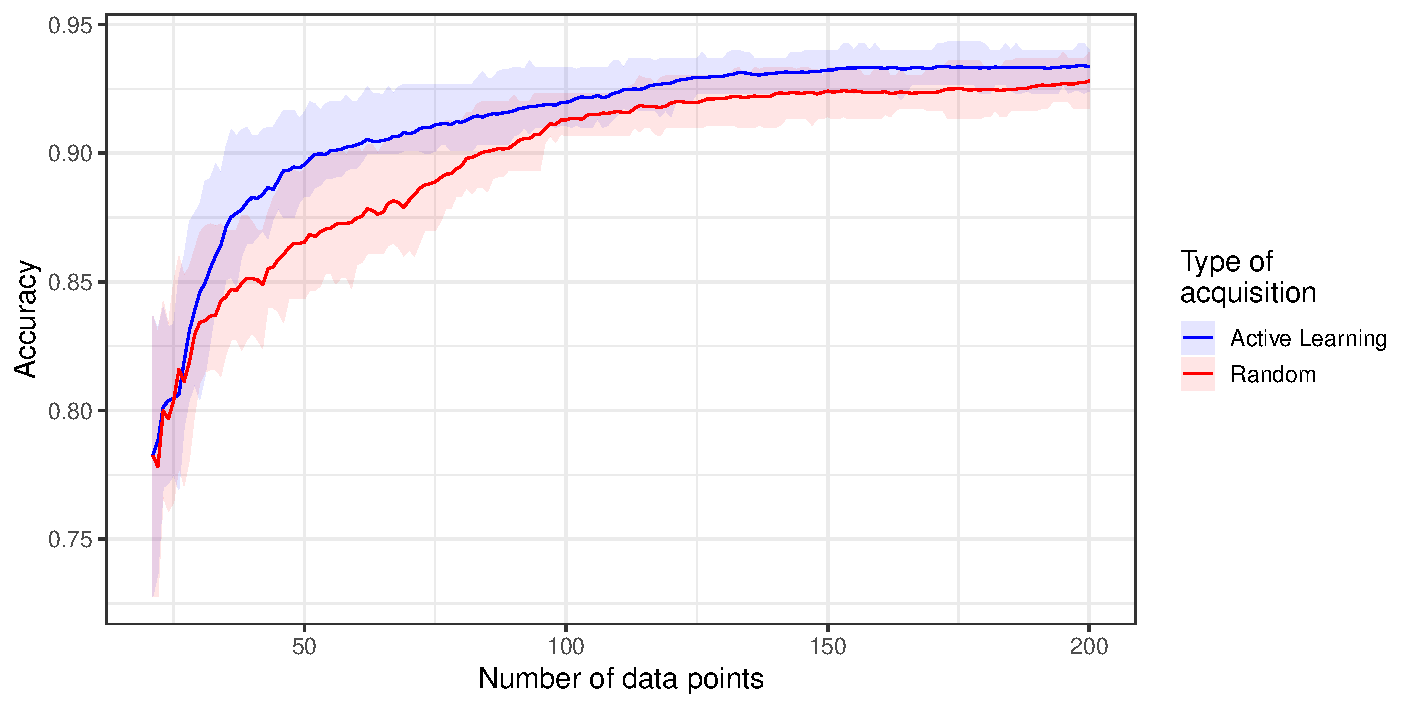
\includegraphics[width=\textwidth]{log_reg_AL_accuracies_plot}
    \caption{Accuracies of a logistic regression model using a variation ratios acquisition function (blue) and a random acquisition function (red).}
    \label{fig:log_reg_AL_accuracies_plot}
\end{figure}


\begin{figure}[H]
    \centering
    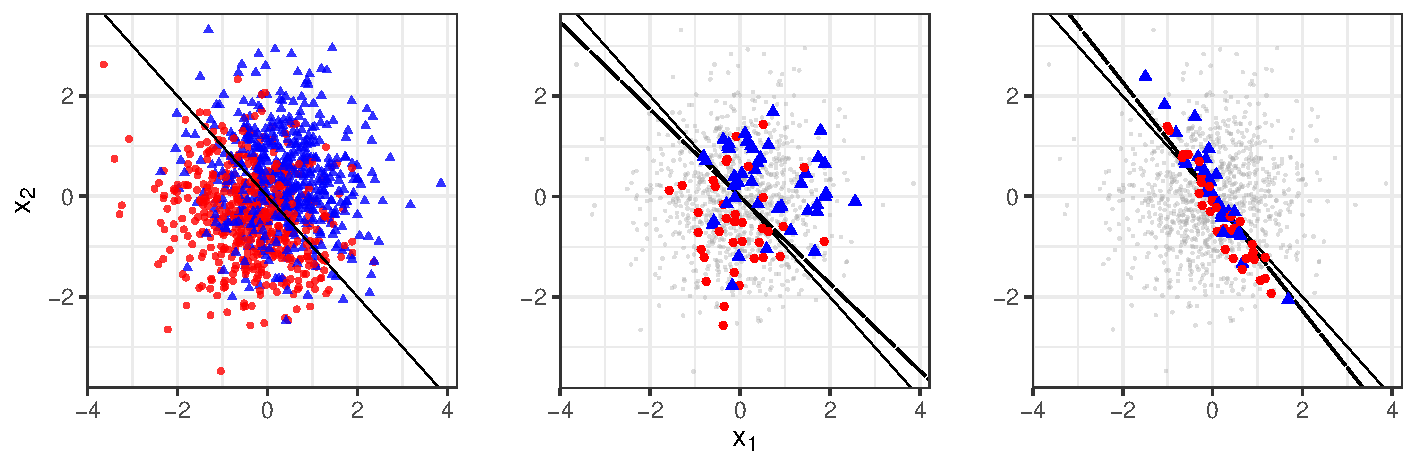
\includegraphics[width=\textwidth]{log_reg_AL_decision_boundary_plot}
    \caption{AL example 1.}
    \label{fig:log_reg_AL_decision_boundary_plot}
\end{figure}
